\section{Modello 2: bagno a collo di bottiglia, free probability e rumore}\label{sec:bottleneck}

\CartoonModelTwo
\subsection{Il modello e la ricorsione esatta}
Seguiamo il modello minimale di Fritzsch e Claeys \cite{FC25}. Ci sono tre siti: il sistema A e il collo di bottiglia C, entrambi di dimensione $d$, e il bagno E, di dimensione $D$. Un passo in avanti consiste di tre operazioni:
\begin{enumerate}[leftmargin=2em]
\item un gate fisso $U$ su A$\otimes$C;
\item un'unitaria Haar indipendente $V_s$ su C$\otimes$E;
\item un canale di rumore, depolarizzante con probabilità $p$, che di default agisce su tutto E.
\end{enumerate}
L'OTOC di ordine $k$ è
\[
C_k(t)=\frac{1}{d^2D}\operatorname{Tr}\bigl[(A(t)B)^k\bigr],
\]
con $A(t)=\Lambda_t^\dagger(A)$ l'evoluzione di Heisenberg rumorosa e $A,B$ operatori sul sito A.

Usiamo la scrittura $\operatorname{Tr}[(A(t)B)^k]=\operatorname{Tr}[A(t)^{\otimes k}B^{\otimes k}P_\gamma]$, con $P_\gamma$ la permutazione ciclica. Ogni copia è una replica, e il rumore agisce copia per copia. Questa è la scelta fisica: in un esperimento a $k$ copie il rumore agisce sulla matrice densità di ciascuna copia.

Dopo la media su ogni $V_s$, l'operatore a $k$ copie ha la forma $\sum_{\tau\in S_k}X_\tau\otimes P_{\tau,\rm C}\otimes P_{\tau,\rm E}$. La ricorsione esatta, valida a ogni $D$, è
\[
X'_{\tau'}=\sum_{\tau,\sigma\in S_k}\mathrm{Wg}(\sigma^{-1}\tau',dD)\;T_{\rm E}(\tau,\sigma)\;\operatorname{Tr}_{\rm C^{\otimes k}}\!\bigl[U^{\dagger\otimes k}(X_\tau\otimes P_{\tau,\rm C})U^{\otimes k}\,P_{\sigma,\rm C}^\dagger\bigr],
\]
con
\[
T_{\rm E}(\tau,\sigma)=\operatorname{Tr}\bigl[\mathcal N^{\dagger\otimes k}(P_\tau)\,P^\dagger_\sigma\bigr],
\]
calcolato in forma chiusa sommando sui sottoinsiemi di copie depolarizzate. La ricorsione è verificata contro il Monte Carlo per $k=2,3$, $D=2,3$, con e senza rumore (\cref{app:num2}).

\subsection{Limite $D\to\infty$ a $k=2$: due settori}
Indichiamo con $\square$ l'etichetta identità (ogni replica tracciata per conto suo) e con $\circ$ lo swap (repliche incrociate, cioè l'eco). Scriviamo $\mathcal U_\tau(X)=U^{\dagger\otimes2}(X\otimes P_{\tau,\rm C})U^{\otimes2}$ e $R_\sigma(Y)=\operatorname{Tr}_{\rm C^{\otimes2}}[Y\,P_{\sigma,\rm C}]$.

All'ordine dominante in $1/D$, e riscalando $\tilde X_\circ=D\,X_\circ$, procedendo in tempo di Heisenberg da $t$ verso $0$ si ha
\begin{align*}
X_\square&\ \leftarrow\ \mathcal M_\square(X_\square)=\tfrac1{d^2}R_e\bigl[\mathcal U_e(X_\square)\bigr]=(\mathcal M^\dagger\otimes\mathcal M^\dagger)(X_\square),\\
\tilde X_\circ&\ \leftarrow\ u\,\mathcal M_\circ(\tilde X_\circ)+\mathcal K(X_\square),\qquad \mathcal M_\circ(X)=\tfrac1{d^2}R_F\bigl[\mathcal U_F(X)\bigr],\qquad \mathcal K(X)=\tfrac1{d^2}\Bigl(R_F-\tfrac1dR_e\Bigr)\bigl[\mathcal U_e(X)\bigr],
\end{align*}
con $u=(1-p)^2$. Qui $\mathcal M^\dagger(X)=\operatorname{Tr}_{\rm C}[U^\dagger(X\otimes I)U]/d$ è il canale a una replica, e il termine $-\tfrac1d R_e$ è il contro-termine di Weingarten. L'OTOC si ottiene come
\[
C_2(t)=\tfrac1{d^2}\operatorname{Tr}\bigl[(Y_\square+\tilde Y_\circ)(B\otimes I)^{\otimes2}F_{\rm AC}\bigr].
\]
Il limite coincide con la ricorsione esatta a $D=10^3$ e $10^5$, a 6 cifre.

\paragraph{Conferme rispetto alle note di lavoro.}
\begin{itemize}[leftmargin=1.5em]
\item Il rumore sul bagno entra \emph{solo} come fattore $u$ davanti a $\mathcal M_\circ$: smorza il settore dell'eco e lascia intatti $\square$ e $\mathcal K$. Questo conferma l'inferenza del \S8 delle note.
\item $\mathcal M_\square$ e $\mathcal M_\circ$ hanno lo stesso spettro, cioè due copie del canale a una replica. La degenerazione produce un blocco di Jordan e il prefattore $t\,\lambda^{2t}$ (per un gate generico con $\lambda=0.462$, il tasso apparente su $t\in[10,20]$ è $0.230\approx\lambda^2(2)^{1/10}$). Qualunque $u<1$ rompe la degenerazione: il prefattore sparisce e il tasso diventa esattamente $\lambda^2$.
\end{itemize}

\begin{figure}[t]
\centering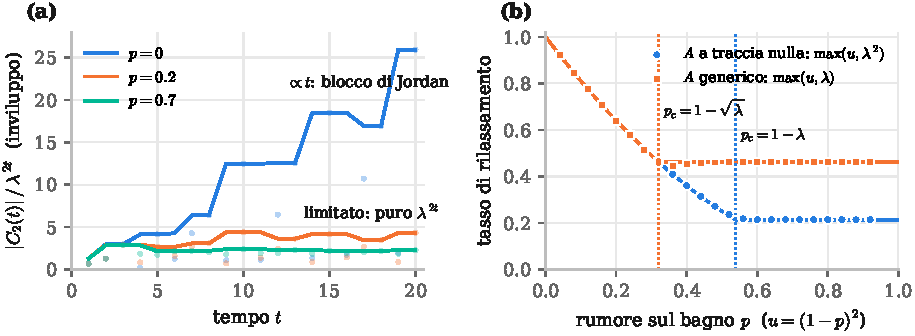
\includegraphics[width=\textwidth]{figs/fig_model2_rates.pdf}
\caption{Modello 2, OTOC a due repliche ($\lambda=0.462$). (a) OTOC compensato $|C_2(t)|/\lambda^{2t}$, con $A=B=Z$; si mostra l'inviluppo delle oscillazioni dovute agli autovalori complessi del canale. Senza rumore cresce linearmente in $t$ (blocco di Jordan); con rumore resta limitato. (b) Tasso di rilassamento asintotico in funzione di $p$. I punti sono la stima numerica su $t\in[14,24]$, le linee sono $\max(u,\lambda^2)$ e $\max(u,\lambda)$, e le verticali segnano gli incroci $p_c$.}
\label{fig:m2rates}
\end{figure}
\begin{figure}[t]
\centering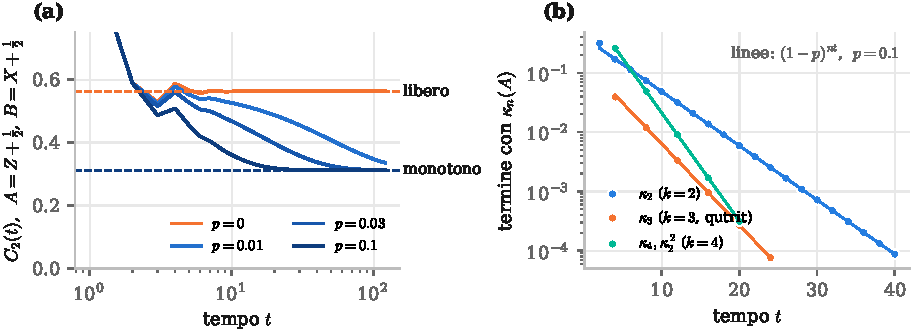
\includegraphics[width=\textwidth]{figs/fig_model2_free.pdf}
\caption{Modello 2, free probability e rumore. (a) $C_2(t)$ per $A=Z+\tfrac12$, $B=X+\tfrac12$: senza rumore tende al valore libero, con qualunque rumore al valore monotono $\varphi(A)^2\varphi(B^2)$. (b) Spettroscopia dei cumulanti a $p=0.1$: il termine proporzionale a $\kappa_n(A)$ decade come $(1-p)^{nt}$ (linee), per $n=2,3,4$.}
\label{fig:m2free}
\end{figure}
\subsection{Risultati}
I risultati sono riassunti nelle \cref{fig:m2rates,fig:m2free}.

\begin{proposition}[valori a tempi lunghi]\label{prop:mono}
Senza rumore, $C_k(\infty)=\sum_{\pi\in NC(k)}\kappa_\pi(A)\,\varphi_{K(\pi)}(B)$: $A(t)$ e $B$ sono liberi. Verificato per $k=2,3$, con qubit e qutrit.

Con qualunque rumore ($p>0$, su E, su C o su A) si ha invece
\[
C_k(\infty)=\varphi(A)^k\,\varphi(B^k).
\]
È la regola dell'indipendenza \emph{monotona} con $A(t)\succ B$. Equivale a dire che, in ogni momento a più repliche, $A(t)\to\varphi(A)\,\mathbb 1$.
\end{proposition}

\begin{proposition}[spettroscopia dei cumulanti liberi]\label{prop:spectro}
Con rumore sul bagno, il contributo a $C_k(t)$ proporzionale a $\kappa_n(A)$ decade come $(1-p)^{nt}$. Numericamente:
\begin{itemize}[leftmargin=1.5em]
\item $n=2$, $k=2$ e $k=3$, $p=0.1$: tasso $0.809$ contro $(0.9)^2=0.81$;
\item $n=3$, $k=3$ con qutrit, $p=0.1$: tasso $0.7290$ contro $(0.9)^3=0.729$.
\end{itemize}
Interpretazione: un cumulante libero di ordine $n$ richiede $n$ copie la cui eco sopravvive, e ogni copia sopravvive al rumore con probabilità $1-p$ per passo.
\end{proposition}

\noindent \emph{Meccanismo.} Il depolarizzante agisce su un'etichetta $\sigma\in S_k$ come
\[
\mathcal N^{\dagger\otimes k}(P_\sigma)=(1-p)^{\,k-\mathrm{fix}(\sigma)}\,P_\sigma+O(1/D),
\]
dove $\mathrm{fix}(\sigma)$ è il numero di punti fissi di $\sigma$. Infatti i sottoinsiemi di copie depolarizzate contenuti nei punti fissi riproducono $P_\sigma$, mentre togliere un punto mosso costa un fattore $1/D$.

Nella formula a multicatene, il termine $\kappa_\pi(A)\varphi_{K(\pi)}(B)$ resta a lungo sull'etichetta $\pi$. Ci aspettiamo quindi che decada come $(1-p)^{(k-\#\text{singoletti}(\pi))\,t}$. Verifica a $k=4$, con $A=Z$ a traccia nulla, $B=X+\tfrac12$ e $p=0.1$: i termini sopravvissuti, $\kappa_4(A)$ e $\kappa_2(A)^2$, spostano tutte e 4 le copie. Il tasso misurato è $0.6561=(1-p)^4$. Senza rumore si riproduce il valore libero $2b^2+b^4=0.5625$. Una dimostrazione per $k$ generico, sul reticolo $NC(k)$, è ancora da scrivere.

\begin{proposition}[incrocio netto dei tassi]\label{prop:cross}
Il rilassamento asintotico di $C_2(t)-C_2(\infty)$ ha tasso
\[
\max\bigl(u,\ \lambda^m\bigr),
\]
con $m=2$ per $A$ a traccia nulla e $m=1$ altrimenti. C'è quindi un incrocio netto in $p_c=1-\lambda^{m/2}$: per il gate di prova, $p_c=0.538$ con $m=2$ e $0.32$ con $m=1$. Vicino all'incrocio compare un prefattore lineare di tipo Jordan. Nelle tabelle in \cref{app:num2}, a $p=0.1$ il tasso misurato è $0.8100=u$, a $p=0.7$ è $0.2140\approx\lambda^2$.
\end{proposition}

\noindent \textbf{Risposta alla domanda Q7 delle note} (crossover o transizione al crescere del rumore). In questo modello il tasso asintotico ha un punto non analitico, quindi la transizione è netta. A tempi finiti è un crossover, con tempo caratteristico $\sim1/(2p)$.

\paragraph{Limiti.} A $D=\infty$ il rumore su una parte \emph{finita} del bagno è irrilevante, perché l'etichetta vive su tutto E. Per il rumore locale nel bagno serve $D$ finito: è esattamente la situazione del modello 1, dove l'incrocio dipende da $pL$. Resta da dimostrare analiticamente la legge $(1-p)^{nt}$ per $k$ generico, sul reticolo $NC(k)$.
